\documentclass[11pt,a4paper]{article}
\usepackage[margin=2.2cm]{geometry}
\usepackage{amsmath,amssymb}
\usepackage{booktabs,longtable,array}
\usepackage{xcolor}
\usepackage{tikz}
\usepackage[export]{adjustbox}
\usetikzlibrary{arrows.meta}
\usepackage{enumitem}
\usepackage[hidelinks]{hyperref}

\begin{filecontents*}[overwrite]{\jobname.bib}
@book{bertsimas1997introduction,
  title     = {Introduction to Linear Optimization},
  author    = {Bertsimas, Dimitris and Tsitsiklis, John N.},
  year      = {1997},
  publisher = {Athena Scientific},
  address   = {Belmont, MA},
  series    = {Athena Scientific Series in Optimization and Neural Computation},
  volume    = {6}
}
@article{picard1976maximal,
  title   = {Maximal Closure of a Graph and Applications to Combinatorial Problems},
  author  = {Picard, Jean-Claude},
  journal = {Management Science},
  volume  = {22},
  number  = {11},
  pages   = {1268--1272},
  year    = {1976}
}
@inproceedings{bienstock2010solving,
  title     = {Solving {LP} Relaxations of Large-Scale Precedence Constrained Problems},
  author    = {Bienstock, Daniel and Zuckerberg, Mark},
  booktitle = {Integer Programming and Combinatorial Optimization (IPCO 2010)},
  series    = {Lecture Notes in Computer Science},
  volume    = {6080},
  pages     = {1--14},
  publisher = {Springer},
  year      = {2010}
}
\end{filecontents*}

\newcolumntype{L}[1]{>{\raggedright\arraybackslash}p{#1}}

\definecolor{cLP}{HTML}{8DB8F2}    % LP foundations
\definecolor{cNET}{HTML}{7FD18B}   % networks
\definecolor{cLS}{HTML}{FFE45C}    % large scale
\definecolor{cCX}{HTML}{FFA64D}    % complexity
\definecolor{cIP}{HTML}{F28B95}    % integer programming
\definecolor{cAP}{HTML}{C3A6EE}    % applications
\definecolor{cMN}{HTML}{C9A27E}    % open-pit mining problems

\title{Reading Plan for Discrete Linear Optimization}
\author{}
\date{}

\begin{document}
\maketitle
\vspace{-1.8cm}

\section*{Reference}
{\small
\begin{verbatim}
@book{bertsimas1997introduction,
  title     = {Introduction to Linear Optimization},
  author    = {Bertsimas, Dimitris and Tsitsiklis, John N.},
  year      = {1997},
  publisher = {Athena Scientific},
  address   = {Belmont, MA},
  series    = {Athena Scientific Series in Optimization and Neural Computation},
  volume    = {6}
}
\end{verbatim}}

\section*{Objective}
This plan selects the parts of~\cite{bertsimas1997introduction} that build
the toolkit of discrete linear optimization. After following it you should
be able to use:
\begin{itemize}[nosep]
  \item \textbf{Polyhedral theory:} extreme points and basic feasible
        solutions, representation of polyhedra, Farkas' lemma.
  \item \textbf{LP algorithms and duality:} simplex and dual simplex, duality
        bounds, reoptimization after adding a variable or a constraint.
  \item \textbf{Large-scale LP:} column generation, constraint generation,
        Dantzig--Wolfe decomposition.
  \item \textbf{Network optimization:} network simplex, max flow/min cut,
        assignment, shortest paths, minimum spanning trees, and the
        integrality of network flows.
  \item \textbf{Integer modeling:} binary-variable formulations and comparison
        of formulations by the strength of their LP relaxations.
  \item \textbf{Exact integer methods:} cutting planes, branch and bound,
        dynamic programming, Lagrangean relaxation.
  \item \textbf{Heuristics:} approximation algorithms, local search,
        simulated annealing.
  \item \textbf{Complexity:} polynomial-time algorithms, separation and the
        ellipsoid method, NP-completeness, to judge which method a problem
        admits.
\end{itemize}
Not covered: Chapter~9, \S2.8, \S3.6--3.7, \S5.2--5.5, \S6.5, \S7.7,
\S12.1--12.2 (1997 edition numbering).

% =====================================================================
\newgeometry{margin=1.2cm,bottom=1.5cm}
\section{Reading paths}
\begin{center}
\adjustbox{max width=\linewidth, max totalheight=0.80\textheight}{%
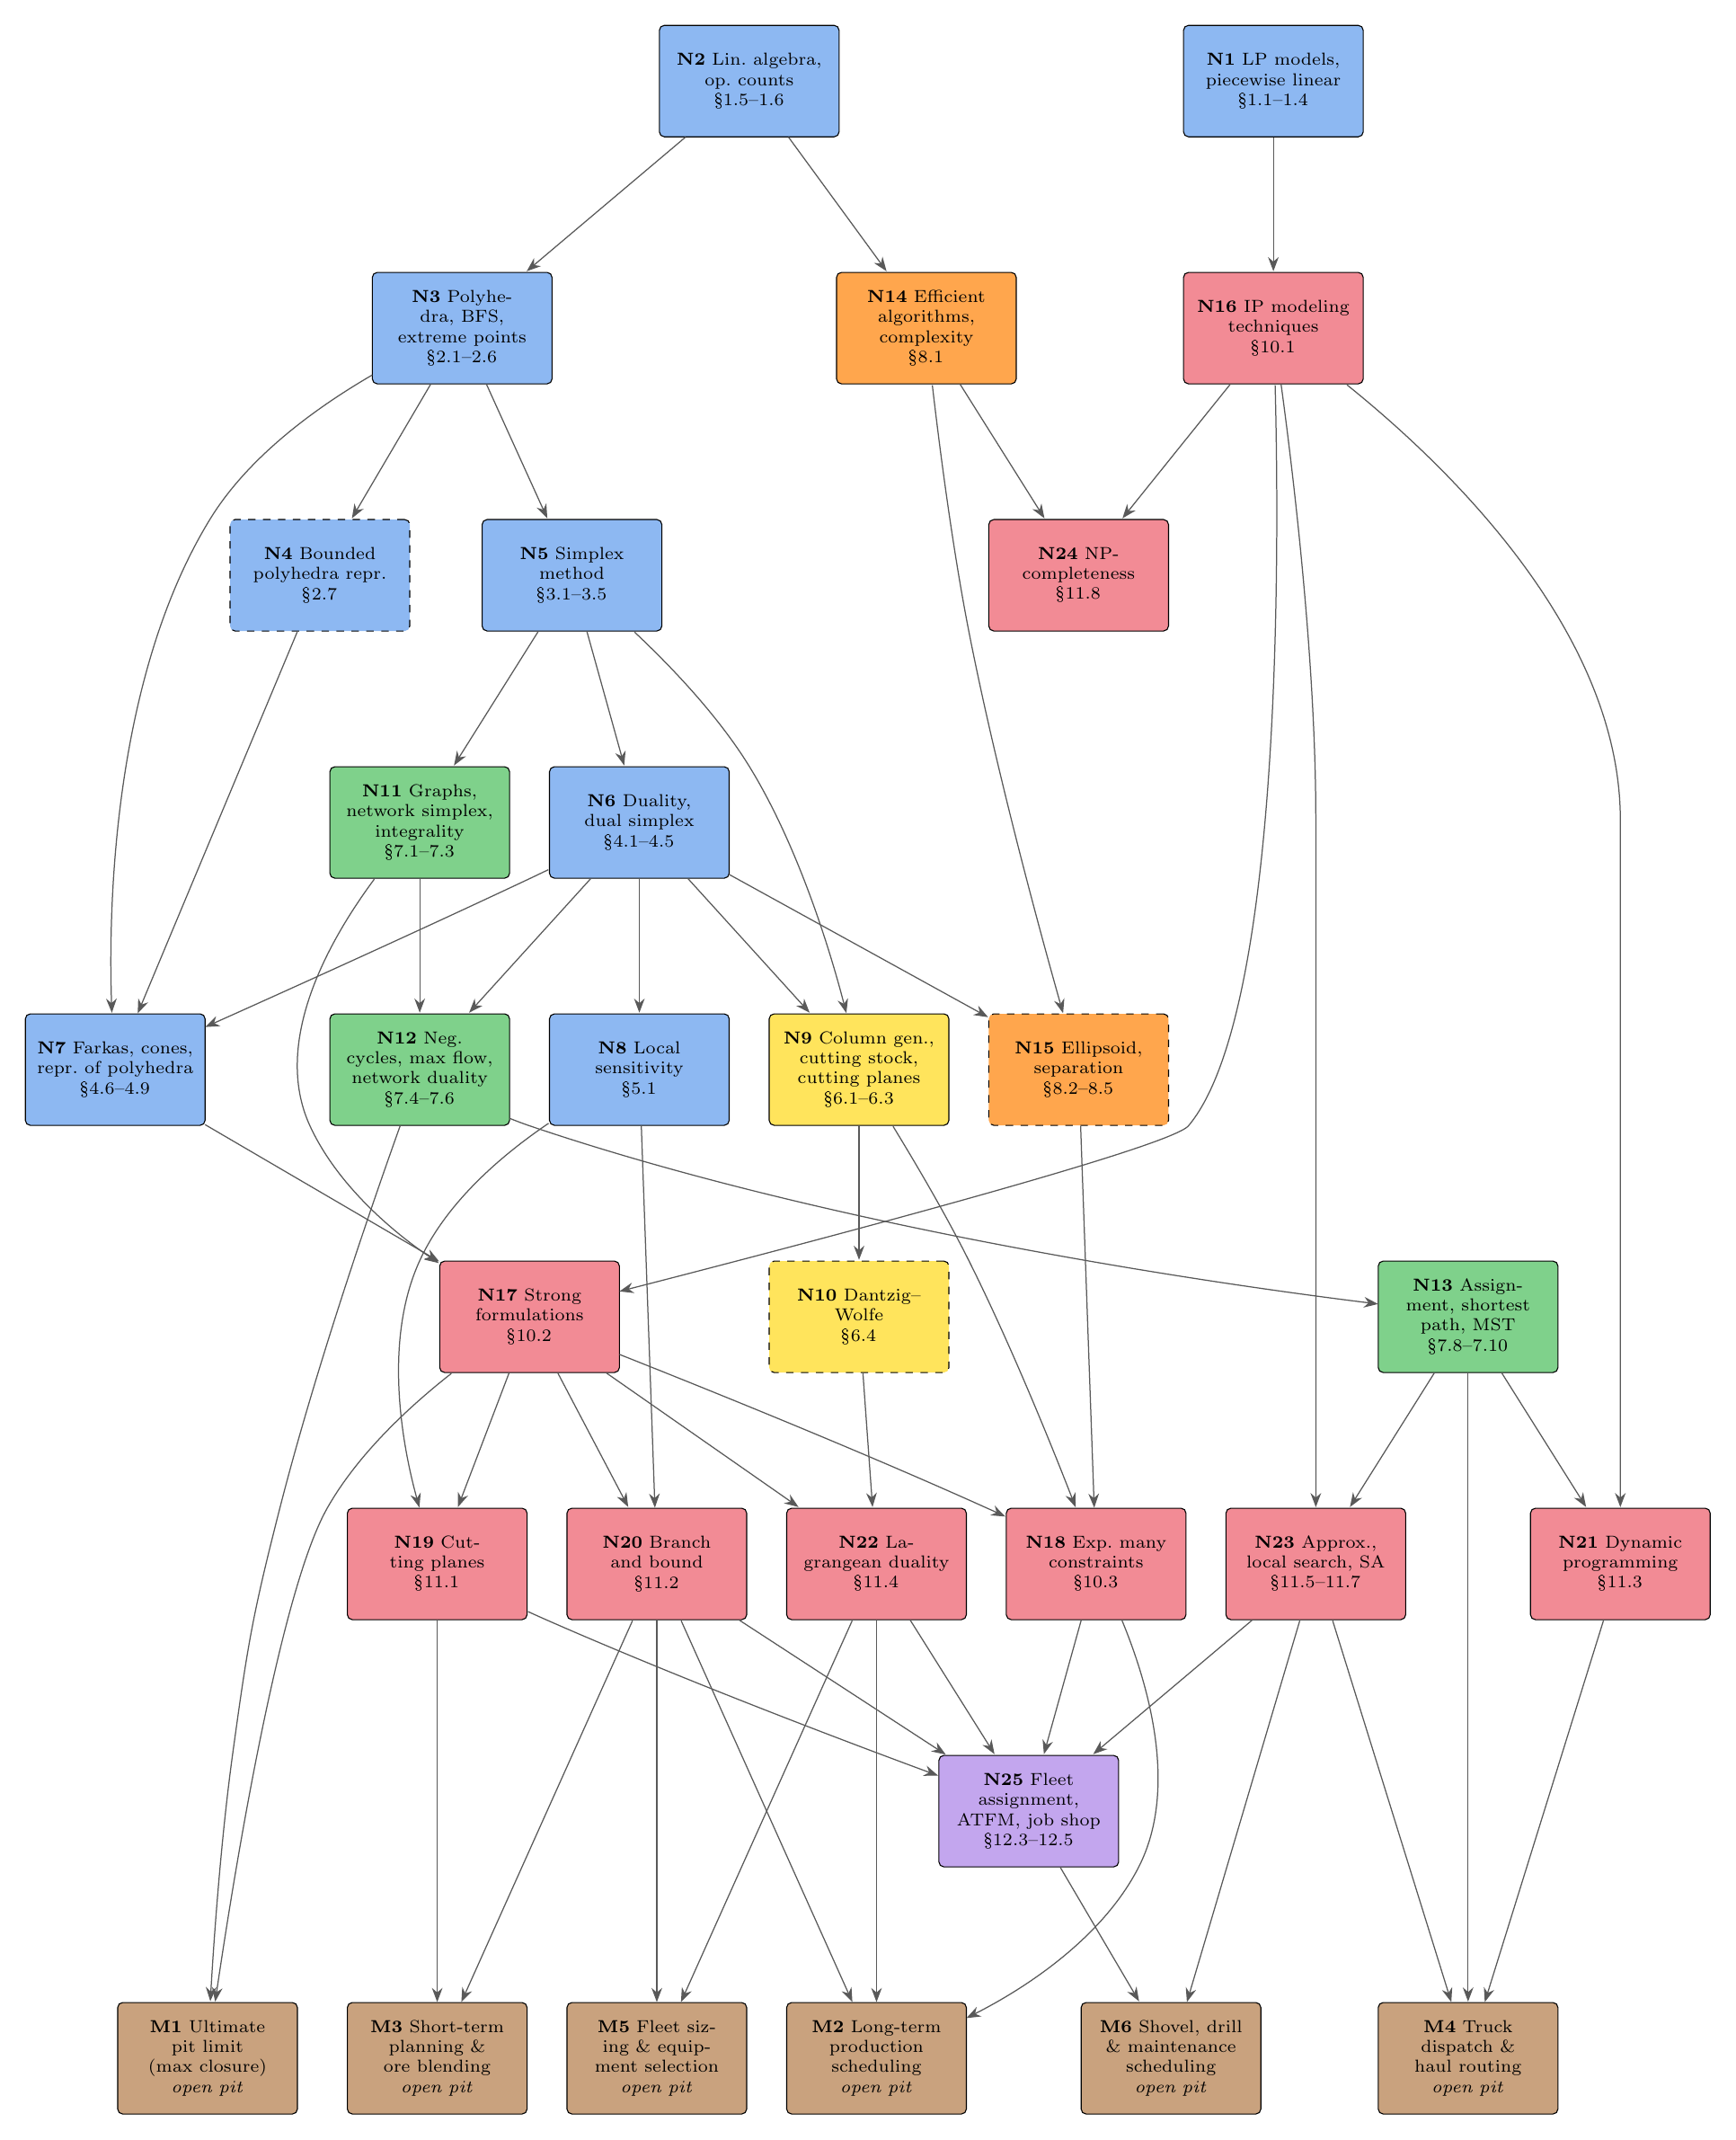
\begin{tikzpicture}[
  nd/.style={draw, rounded corners=2pt, align=center, font=\scriptsize,
             text width=2.3cm, minimum width=2.54cm, minimum height=1.575cm,
             inner sep=2pt},
  opt/.style={dashed},
  lvl/.style={font=\small\bfseries, text=gray},
  ed/.style={-{Stealth[length=2mm]}, gray!70!black, line width=0.45pt},
]
\node[nd,fill=cLP] (N1) at (17.639,28.732) {\textbf{N1} LP models, piecewise linear\\ \S1.1--1.4};
\node[nd,fill=cLP] (N2) at (10.231,28.732) {\textbf{N2} Lin.\ algebra, op.\ counts\\ \S1.5--1.6};
\node[nd,fill=cLP] (N3) at (6.174,25.241) {\textbf{N3} Polyhedra, BFS, extreme points\\ \S2.1--2.6};
\node[nd,fill=cLP,opt] (N4) at (4.163,21.749) {\textbf{N4} Bounded polyhedra repr.\\ \S2.7};
\node[nd,fill=cLP] (N5) at (7.726,21.749) {\textbf{N5} Simplex method\\ \S3.1--3.5};
\node[nd,fill=cLP] (N6) at (8.678,18.256) {\textbf{N6} Duality, dual simplex\\ \S4.1--4.5};
\node[nd,fill=cLP] (N7) at (1.270,14.764) {\textbf{N7} Farkas, cones, repr.\ of polyhedra\\ \S4.6--4.9};
\node[nd,fill=cLP] (N8) at (8.678,14.764) {\textbf{N8} Local sensitivity\\ \S5.1};
\node[nd,fill=cLS] (N9) at (11.783,14.764) {\textbf{N9} Column gen., cutting stock, cutting planes\\ \S6.1--6.3};
\node[nd,fill=cLS,opt] (N10) at (11.783,11.271) {\textbf{N10} Dantzig--Wolfe\\ \S6.4};
\node[nd,fill=cNET] (N11) at (5.574,18.256) {\textbf{N11} Graphs, network simplex, integrality\\ \S7.1--7.3};
\node[nd,fill=cNET] (N12) at (5.574,14.764) {\textbf{N12} Neg.\ cycles, max flow, network duality\\ \S7.4--7.6};
\node[nd,fill=cNET] (N13) at (20.391,11.271) {\textbf{N13} Assignment, shortest path, MST\\ \S7.8--7.10};
\node[nd,fill=cCX] (N14) at (12.735,25.241) {\textbf{N14} Efficient algorithms, complexity\\ \S8.1};
\node[nd,fill=cCX,opt] (N15) at (14.887,14.764) {\textbf{N15} Ellipsoid, separation\\ \S8.2--8.5};
\node[nd,fill=cIP] (N16) at (17.639,25.241) {\textbf{N16} IP modeling techniques\\ \S10.1};
\node[nd,fill=cIP] (N17) at (7.126,11.271) {\textbf{N17} Strong formulations\\ \S10.2};
\node[nd,fill=cIP] (N18) at (15.134,7.779) {\textbf{N18} Exp.\ many constraints\\ \S10.3};
\node[nd,fill=cIP] (N19) at (5.821,7.779) {\textbf{N19} Cutting planes\\ \S11.1};
\node[nd,fill=cIP] (N20) at (8.925,7.779) {\textbf{N20} Branch and bound\\ \S11.2};
\node[nd,fill=cIP] (N21) at (22.543,7.779) {\textbf{N21} Dynamic programming\\ \S11.3};
\node[nd,fill=cIP] (N22) at (12.030,7.779) {\textbf{N22} Lagrangean duality\\ \S11.4};
\node[nd,fill=cIP] (N23) at (18.239,7.779) {\textbf{N23} Approx., local search, SA\\ \S11.5--11.7};
\node[nd,fill=cIP] (N24) at (14.887,21.749) {\textbf{N24} NP-completeness\\ \S11.8};
\node[nd,fill=cAP] (N25) at (14.182,4.286) {\textbf{N25} Fleet assignment, ATFM, job shop\\ \S12.3--12.5};
\node[nd,fill=cMN] (M1) at (2.575,0.794) {\textbf{M1} Ultimate pit limit (max closure)\\ \emph{open pit}};
\node[nd,fill=cMN] (M2) at (12.030,0.794) {\textbf{M2} Long-term production scheduling\\ \emph{open pit}};
\node[nd,fill=cMN] (M3) at (5.821,0.794) {\textbf{M3} Short-term planning \& ore blending\\ \emph{open pit}};
\node[nd,fill=cMN] (M4) at (20.391,0.794) {\textbf{M4} Truck dispatch \& haul routing\\ \emph{open pit}};
\node[nd,fill=cMN] (M5) at (8.925,0.794) {\textbf{M5} Fleet sizing \& equipment selection\\ \emph{open pit}};
\node[nd,fill=cMN] (M6) at (16.192,0.794) {\textbf{M6} Shovel, drill \& maintenance scheduling\\ \emph{open pit}};
\draw[ed] (17.639,27.940) .. controls (17.639,27.376) and (17.639,26.612) .. (17.639,26.045);
\draw[ed] (9.330,27.940) .. controls (8.663,27.376) and (7.756,26.612) .. (7.086,26.045);
\draw[ed] (10.786,27.940) .. controls (11.199,27.376) and (11.758,26.612) .. (12.172,26.045);
\draw[ed] (5.727,24.446) .. controls (5.396,23.883) and (4.947,23.119) .. (4.615,22.553);
\draw[ed] (6.518,24.446) .. controls (6.773,23.883) and (7.120,23.119) .. (7.377,22.553);
\draw[ed] (4.903,24.579) .. controls (4.117,24.123) and (3.156,23.431) .. (2.611,22.543) .. controls (1.234,20.298) and (1.171,17.037) .. (1.223,15.567);
\draw[ed] (13.213,24.446) .. controls (13.567,23.883) and (14.048,23.119) .. (14.404,22.553);
\draw[ed] (12.819,24.434) .. controls (12.918,23.579) and (13.099,22.162) .. (13.335,20.955) .. controls (13.720,18.992) and (14.339,16.718) .. (14.667,15.561);
\draw[ed] (17.028,24.446) .. controls (16.575,23.883) and (15.960,23.119) .. (15.506,22.553);
\draw[ed] (17.664,24.433) .. controls (17.723,22.160) and (17.772,15.554) .. (16.439,13.970) .. controls (16.175,13.656) and (10.883,12.268) .. (8.396,11.630);
\draw[ed] (18.679,24.440) .. controls (20.118,23.283) and (22.543,20.941) .. (22.543,18.292) .. controls (22.543,18.292) and (22.543,18.292) .. (22.543,14.728) .. controls (22.543,12.496) and (22.543,9.857) .. (22.543,8.581);
\draw[ed] (17.749,24.440) .. controls (17.922,23.167) and (18.239,20.533) .. (18.239,18.292) .. controls (18.239,18.292) and (18.239,18.292) .. (18.239,14.728) .. controls (18.239,12.496) and (18.239,9.857) .. (18.239,8.581);
\draw[ed] (3.842,20.947) .. controls (3.285,19.614) and (2.143,16.886) .. (1.588,15.558);
\draw[ed] (7.937,20.954) .. controls (8.094,20.391) and (8.307,19.626) .. (8.464,19.061);
\draw[ed] (7.248,20.954) .. controls (6.894,20.391) and (6.413,19.626) .. (6.058,19.061);
\draw[ed] (8.610,20.946) .. controls (9.139,20.449) and (9.791,19.763) .. (10.231,19.050) .. controls (10.923,17.926) and (11.375,16.447) .. (11.604,15.562);
\draw[ed] (7.392,17.589) .. controls (7.302,17.546) and (7.213,17.503) .. (7.126,17.462) .. controls (5.555,16.722) and (3.732,15.898) .. (2.543,15.366);
\draw[ed] (8.678,17.461) .. controls (8.678,16.898) and (8.678,16.134) .. (8.678,15.568);
\draw[ed] (9.367,17.461) .. controls (9.878,16.898) and (10.572,16.134) .. (11.085,15.568);
\draw[ed] (7.989,17.461) .. controls (7.479,16.898) and (6.785,16.134) .. (6.272,15.568);
\draw[ed] (9.950,17.520) .. controls (11.018,16.932) and (12.536,16.095) .. (13.607,15.505);
\draw[ed] (5.574,17.461) .. controls (5.574,16.898) and (5.574,16.134) .. (5.574,15.568);
\draw[ed] (4.931,17.454) .. controls (4.291,16.591) and (3.477,15.155) .. (4.022,13.970) .. controls (4.398,13.151) and (5.165,12.489) .. (5.843,12.030);
\draw[ed] (2.541,13.986) .. controls (3.520,13.414) and (4.867,12.627) .. (5.848,12.054);
\draw[ed] (7.395,14.005) .. controls (6.718,13.546) and (5.950,12.884) .. (5.574,12.065) .. controls (5.055,10.936) and (5.324,9.458) .. (5.569,8.576);
\draw[ed] (8.706,13.962) .. controls (8.753,12.629) and (8.851,9.901) .. (8.898,8.573);
\draw[ed] (11.783,13.969) .. controls (11.783,13.406) and (11.783,12.641) .. (11.783,12.076);
\draw[ed] (12.264,13.962) .. controls (12.585,13.437) and (13.007,12.721) .. (13.335,12.065) .. controls (13.930,10.875) and (14.510,9.441) .. (14.844,8.580);
\draw[ed] (6.851,14.073) .. controls (6.943,14.036) and (7.035,14.001) .. (7.126,13.970) .. controls (11.398,12.524) and (16.723,11.749) .. (19.119,11.452);
\draw[ed] (5.297,13.969) .. controls (4.885,12.816) and (4.103,10.546) .. (3.598,8.572) .. controls (3.207,7.041) and (3.143,6.646) .. (2.928,5.080) .. controls (2.762,3.869) and (2.663,2.453) .. (2.614,1.600);
\draw[ed] (14.915,13.962) .. controls (14.962,12.629) and (15.060,9.901) .. (15.107,8.573);
\draw[ed] (11.838,10.476) .. controls (11.878,9.913) and (11.933,9.149) .. (11.974,8.583);
\draw[ed] (20.868,10.476) .. controls (21.222,9.913) and (21.703,9.149) .. (22.059,8.583);
\draw[ed] (19.913,10.476) .. controls (19.559,9.913) and (19.078,9.149) .. (18.722,8.583);
\draw[ed] (20.391,10.471) .. controls (20.391,8.546) and (20.391,3.521) .. (20.391,1.595);
\draw[ed] (8.398,10.739) .. controls (9.707,10.220) and (11.802,9.374) .. (13.582,8.572) .. controls (13.670,8.533) and (13.759,8.492) .. (13.850,8.449);
\draw[ed] (6.836,10.476) .. controls (6.622,9.913) and (6.330,9.149) .. (6.114,8.583);
\draw[ed] (7.526,10.476) .. controls (7.821,9.913) and (8.224,9.149) .. (8.521,8.583);
\draw[ed] (8.214,10.476) .. controls (9.021,9.913) and (10.117,9.149) .. (10.928,8.583);
\draw[ed] (6.020,10.470) .. controls (5.413,9.993) and (4.698,9.327) .. (4.269,8.572) .. controls (3.586,7.374) and (2.934,3.303) .. (2.683,1.594);
\draw[ed] (14.923,6.984) .. controls (14.766,6.421) and (14.553,5.656) .. (14.396,5.091);
\draw[ed] (15.501,6.977) .. controls (15.868,6.089) and (16.305,4.607) .. (15.734,3.493) .. controls (15.226,2.502) and (14.160,1.797) .. (13.301,1.362);
\draw[ed] (7.104,7.106) .. controls (7.195,7.064) and (7.285,7.024) .. (7.373,6.985) .. controls (9.273,6.151) and (11.523,5.296) .. (12.902,4.787);
\draw[ed] (5.821,6.977) .. controls (5.821,5.644) and (5.821,2.916) .. (5.821,1.588);
\draw[ed] (10.092,6.984) .. controls (10.960,6.419) and (12.140,5.651) .. (13.009,5.085);
\draw[ed] (9.269,6.977) .. controls (9.868,5.644) and (11.093,2.916) .. (11.689,1.588);
\draw[ed] (8.581,6.977) .. controls (7.983,5.644) and (6.758,2.916) .. (6.162,1.588);
\draw[ed] (8.925,6.977) .. controls (8.925,5.644) and (8.925,2.916) .. (8.925,1.588);
\draw[ed] (22.304,6.977) .. controls (21.889,5.644) and (21.040,2.916) .. (20.627,1.588);
\draw[ed] (12.507,6.984) .. controls (12.862,6.421) and (13.342,5.656) .. (13.698,5.091);
\draw[ed] (12.030,6.977) .. controls (12.030,5.644) and (12.030,2.916) .. (12.030,1.588);
\draw[ed] (11.686,6.977) .. controls (11.087,5.644) and (9.862,2.916) .. (9.266,1.588);
\draw[ed] (17.338,6.984) .. controls (16.671,6.421) and (15.764,5.656) .. (15.093,5.091);
\draw[ed] (18.477,6.977) .. controls (18.892,5.644) and (19.741,2.916) .. (20.154,1.588);
\draw[ed] (18.012,6.977) .. controls (17.617,5.644) and (16.810,2.916) .. (16.417,1.588);
\draw[ed] (14.628,3.491) .. controls (14.959,2.928) and (15.408,2.164) .. (15.741,1.598);
\end{tikzpicture}}
\end{center}

\noindent\textbf{Legend.}
\colorbox{cLP}{LP foundations}\,
\colorbox{cNET}{Networks}\,
\colorbox{cLS}{Large scale}\,
\colorbox{cCX}{Complexity}\,
\colorbox{cIP}{Integer programming}\,
\colorbox{cAP}{Book applications}\,
\colorbox{cMN}{Open-pit mining (outside the book)}.
Dashed box: optional, can be dropped if time is short.
\restoregeometry

% =====================================================================
% =====================================================================
\section{Node coverage table}
Hours: estimated time to read the sections and solve a few exercises per node. Total: 191 hours.
\footnotesize
\begin{longtable}{@{}l L{1.5cm} L{4.9cm} L{4.9cm} c l@{}}
\toprule
\textbf{Node} & \textbf{Sections} & \textbf{Content covered} & \textbf{Role in discrete optimization} & \textbf{Hours} & \textbf{Status}\\
\midrule
\endhead
\bottomrule
\endfoot
N1 & 1.1--1.4 & LP forms, modeling examples, piecewise linear convex objectives, graphical solution & Modeling vocabulary reused for IP & 4 & Core\\
N2 & 1.5--1.6 & Notation, linear algebra, operation counts & Basis for complexity arguments & 4 & Support\\
N3 & 2.1--2.6 & Polyhedra, extreme points $=$ vertices $=$ BFS, degeneracy, optimality of extreme points & Integrality is a question about extreme points & 12 & Core\\
N14 & 8.1 & Input size, polynomial vs.\ exponential algorithms & Prerequisite for NP-completeness & 3 & Core\\
N16 & 10.1 & Binary choice, forcing constraints, disjunctions, piecewise linear costs & Turning logic into linear constraints & 5 & Core\\
N4 & 2.7 & Bounded polyhedron $=$ convex hull of extreme points & Underlies $\mathrm{conv}(S)$ & 3 & Optional\\
N5 & 3.1--3.5 & Reduced costs, simplex, tableau, anticycling, Phase I & Tableau used by Gomory cuts and network simplex & 16 & Core\\
N24 & 11.8 & P, NP, NP-completeness, reductions & Explains why IP is hard & 8 & Core\\
N6 & 4.1--4.5 & Duality, complementary slackness, shadow prices, dual simplex & Bounds, reoptimization, network duality & 16 & Core\\
N11 & 7.1--7.3 & Graphs, network flow formulation, network simplex, integral flows & Integer problems solvable as LPs & 10 & Core\\
N7 & 4.6--4.9 & Farkas' lemma, cones, extreme rays, resolution theorem & Polyhedral description of $\mathrm{conv}(S)$ & 10 & Core\\
N8 & 5.1 & Adding a variable/constraint, changes in $b$, $c$ & The operations of cutting and branching & 5 & Core\\
N9 & 6.1--6.3 & Column generation, cutting stock, constraint generation & Large formulations; prototype of separation & 8 & Core\\
N12 & 7.4--7.6 & Negative cost cycles, max flow, min cut, network duality & Min--max theorems via LP duality & 8 & Core\\
N15 & 8.2--8.5 & Ellipsoid method, separation, exponentially many constraints & Separation $\equiv$ optimization & 6 & Optional\\
N10 & 6.4 & Dantzig--Wolfe decomposition & Linked to Lagrangean duality & 5 & Optional\\
N13 & 7.8--7.10 & Assignment, auction, shortest path, MST & Combinatorial subproblems & 8 & Core\\
N17 & 10.2 & Comparing formulations; ideal formulation $=\mathrm{conv}(S)$ & Central concept of the plan & 12 & Core\\
N18 & 10.3 & Formulations with exponentially many constraints & Needs separation/cutting planes & 6 & Core\\
N19 & 11.1 & Gomory cutting planes & Exact method from tableau rows & 6 & Core\\
N20 & 11.2 & Branch and bound & Workhorse algorithm for IP & 10 & Core\\
N21 & 11.3 & Dynamic programming (knapsack) & Pseudo-polynomial exact method & 4 & Core\\
N22 & 11.4 & Lagrangean relaxation and dual & Stronger bounds than LP & 10 & Core\\
N23 & 11.5--11.7 & Approximation, local search, simulated annealing & Methods for large instances & 6 & Support\\
N25 & 12.3--12.5 & Fleet assignment, air traffic flow, job shop & Formulation $+$ methods together & 6 & Support\\
\end{longtable}
\normalsize

\section{Open-pit mining problems}
The bottom nodes of the graph (M1--M6) are open-pit mining problems that the techniques above can solve. For each one: the path in the graph that leads to it, what the problem asks, and why it needs the nodes with a direct arrow into it.

\begin{description}[leftmargin=0pt, style=nextline]
\item[Ultimate pit limit (M1).]
  Path in the graph: N2 $\to$ N3 $\to$ N5 $\to$ N11 $\to$ N12 $\to$ M1, with N7 $\to$ N17 $\to$ M1.\\
  \emph{Objective:} the most valuable set of blocks that respects slope precedence.\\
  \emph{Why the parents:} the problem is a maximum closure, which reduces to a
  minimum cut~\cite{picard1976maximal}; N12 gives max-flow/min-cut. N17
  explains why the precedence formulation is already ideal, so the LP
  relaxation returns an integer pit without branching.

\item[Long-term production scheduling (M2).]
  Path in the graph: N6 $\to$ N9 $\to$ N10 $\to$ N22 $\to$ M2, with N17 $\to$ N18 $\to$ M2 and N17 $\to$ N20 $\to$ M2.\\
  \emph{Objective:} assign blocks to periods to maximize NPV under precedence
  and capacity.\\
  \emph{Why the parents:} N18 handles the huge number of precedence
  constraints; N22 relaxes capacities so each subproblem becomes a pit
  (closure) problem, which gives bounds~\cite{bienstock2010solving}; N20
  closes the remaining integrality gap.

\item[Short-term planning and ore blending (M3).]
  Path in the graph: N5 $\to$ N6 $\to$ N8 $\to$ N19, N20 $\to$ M3, with N17 $\to$ N19, N20.\\
  \emph{Objective:} choose faces or polygons per week or shift that meet
  tonnage and grade bounds.\\
  \emph{Why the parents:} N19 strengthens the relaxation with cuts; N20 fixes
  the binary extraction decisions; both rely on N8 to reoptimize after adding
  a cut or a branch.

\item[Truck dispatching and haul routing (M4).]
  Path in the graph: N11 $\to$ N12 $\to$ N13 $\to$ M4, with N13 $\to$ N21, N23 $\to$ M4.\\
  \emph{Objective:} assign trucks to shovels and dumps, and pick haul routes,
  in real time.\\
  \emph{Why the parents:} N13 gives shortest paths (routes) and assignment
  (truck--shovel); N21 models sequential decisions, the bridge to stochastic
  DP and RL; N23 gives fast heuristics when exact solutions are too slow.

\item[Fleet sizing and equipment selection (M5).]
  Path in the graph: N17 $\to$ N20 $\to$ M5, with N9 $\to$ N10 $\to$ N22 $\to$ M5.\\
  \emph{Objective:} integer numbers of trucks and shovels per period at minimum cost.\\
  \emph{Why the parents:} N20 handles the integer fleet counts; N22 decomposes
  the problem by period and gives lower bounds.

\item[Shovel, drill and maintenance scheduling (M6).]
  Path in the graph: N20, N22, N18, N19, N23 $\to$ N25 $\to$ M6, with N23 $\to$ M6.\\
  \emph{Objective:} sequence equipment moves and maintenance windows.\\
  \emph{Why the parents:} N25 (\S12.5, job shop) gives the scheduling
  formulation; such problems are NP-hard, so N23 supplies the heuristics used
  in practice.
\end{description}

\bibliographystyle{plain}
\bibliography{\jobname}
\end{document}
